\documentclass[review]{elsarticle}

\usepackage{multirow}
\usepackage{lineno}
\usepackage{xspace}
\usepackage{threeparttable}
\usepackage[T1]{fontenc}
\usepackage{lmodern}
\modulolinenumbers[5]

%% Journal name here
\journal{Nuclear Technology}

%% `Elsevier LaTeX' style
\bibliographystyle{elsarticle-num}
%%%%%%%%%%%%%%%%%%%%%%%

%%%% packages and definitions (optional)
\usepackage{placeins}
\usepackage{booktabs} % nice rules (thick lines) for tables
\usepackage{microtype} % improves typography for PDF
\usepackage{hhline}
\usepackage{amsmath}
\usepackage{caption}
\usepackage{subcaption}

\usepackage{booktabs}
\usepackage{threeparttable, tablefootnote}

\usepackage{tabularx}

%% Special typesetting for Cyclus
\newcommand{\Cyclus}{\textsc{Cyclus}\xspace}%
\newcommand{\Cycamore}{\textsc{Cycamore}\xspace}%
\newcommand{\keff}{$k_{eff}$\xspace}
\newcommand{\betaEff}{$\beta_{eff}$\xspace}
\graphicspath{{images/}}

% tikz %
\usepackage{tikz}
\usetikzlibrary{positioning, arrows, decorations, shapes}

\usetikzlibrary{shapes.geometric,arrows}
\tikzstyle{process} = [rectangle, rounded corners, minimum width=3cm, minimum height=1cm,text centered, draw=black, fill=blue!30]
\tikzstyle{object} = [ellipse, rounded corners, minimum width=3cm, minimum height=1cm,text centered, draw=black, fill=green!30]
\tikzstyle{arrow} = [thick,->,>=stealth]

% hyperref %
\usepackage[hidelinks]{hyperref}
% after hyperref %
\usepackage{cleveref}
\usepackage{datatool}
\usepackage[acronym,toc]{glossaries}
\newacronym[longplural={metric tons of heavy metal}]{MTHM}{MTHM}{metric ton of heavy metal}
\newacronym{ABM}{ABM}{agent-based modeling}
\newacronym{ACDIS}{ACDIS}{Program in Arms Control \& Domestic and International Security}
\newacronym{AFCI}{AFCI}{Advanced Fuel Cycle Initiative}
\newacronym{AHTR}{AHTR}{Advanced High Temperature Reactor}
\newacronym{ANDRA}{ANDRA}{Agence Nationale pour la gestion des D\'echets RAdioactifs, the French National Agency for Radioactive Waste Management}
\newacronym{ANL}{ANL}{Argonne National Laboratory}
\newacronym{ARDP}{ARDP}{Advanced Reactors Demonstration Program}
\newacronym{API}{API}{application programming interface}
\newacronym{ARCH}{ARCH}{autoregressive conditional heteroskedastic}
\newacronym{ARE}{ARE}{Aircraft Reactor Experiment}
\newacronym{ARFC}{ARFC}{Advanced Reactors and Fuel Cycles}
\newacronym{ARMA}{ARMA}{autoregressive moving average}
\newacronym{ASME}{ASME}{American Society of Mechanical Engineers}
\newacronym{ATWS}{ATWS}{Anticipated Transient Without Scram}
\newacronym{BDBE}{BDBE}{Beyond Design Basis Event}
\newacronym{BIDS}{BIDS}{Berkeley Institute for Data Science}
\newacronym{BOL}{BOL}{Beginning-of-Life}
\newacronym{BSD}{BSD}{Berkeley Software Distribution}
\newacronym{BWR}{BWR}{Boiling Water Reactor}
\newacronym{CAFCA}{CAFCA}{ Code for Advanced Fuel Cycles Assessment }
\newacronym{CASL}{CASL}{Consortium for Advanced Simulation of Light Water Reactors}
\newacronym{CDTN}{CDTN}{Centro de Desenvolvimento da Tecnologia Nuclear}
\newacronym{CEA}{CEA}{Commissariat \`a l'\'Energie Atomique et aux \'Energies Alternatives}
\newacronym{CI}{CI}{continuous integration}
\newacronym{CLASS}{CLASS}{Core Library for Advanced Scenario Simulation}
\newacronym{CNEC}{CNEC}{Consortium for Nonproliferation Enabling Capabilities}
\newacronym{CNEN}{CNEN}{Comiss\~{a}o Nacional de Energia Nuclear}
\newacronym{CNERG}{CNERG}{Computational Nuclear Engineering Research Group}
\newacronym{COSI}{COSI}{Commelini-Sicard}
\newacronym{COTS}{COTS}{commercial, off-the-shelf}
\newacronym{CRAM}{CRAM}{Chebyshev rational approximation method}
\newacronym{CSNF}{CSNF}{commercial spent nuclear fuel}
\newacronym{CTAH}{CTAHs}{Coiled Tube Air Heaters}
\newacronym{CUBIT}{CUBIT}{CUBIT Geometry and Mesh Generation Toolkit}
\newacronym{CURIE}{CURIE}{Centralized Used Fuel Resource for Information Exchange}
\newacronym{CYBORG}{CyBORG}{Cyclus-Based ORiGen}
\newacronym{DAG}{DAG}{directed acyclic graph}
\newacronym{DANESS}{DANESS}{Dynamic Analysis of Nuclear Energy System Strategies}
\newacronym{DBE}{DBE}{Design Basis Event}
\newacronym{DESAE}{DESAE}{Dynamic Analysis of Nuclear Energy Systems Strategies}
\newacronym{DHS}{DHS}{Department of Homeland Security}
\newacronym{DOE}{DOE}{Department of Energy}
\newacronym{DOE-NE}{DOE-NE}{U.S. Department of Energy, Office of Nuclear Energy}
\newacronym{DRACS}{DRACS}{Direct Reactor Auxiliary Cooling System}
\newacronym{DRE}{DRE}{dynamic resource exchange}
\newacronym{DSNF}{DSNF}{DOE spent nuclear fuel}
\newacronym{DYMOND}{DYMOND}{Dynamic Model of Nuclear Development }
\newacronym{EBS}{EBS}{Engineered Barrier System}
\newacronym{EBR}{EBR-II}{Experimental Breeder Reactor II}
\newacronym{EDZ}{EDZ}{Excavation Disturbed Zone}
\newacronym{EG}{EG}{Evaluation Group}
\newacronym{EIA}{EIA}{U.S. Energy Information Administration}
\newacronym{EOL}{EOL}{End-of-life}
\newacronym{EPA}{EPA}{Environmental Protection Agency}
\newacronym{EP}{EP}{Engineering Physics}
\newacronym{ES}{E\&S}{Evaluation and Screening}
\newacronym{FCM}{FCM}{Fully Ceramic Microencapsulated}
\newacronym{FCO}{FCO}{Fuel Cycle Options}
\newacronym{FCT}{FCT}{Fuel Cycle Technology}
\newacronym{FCWMD}{FCWMD}{Fuel Cycle and Waste Management Division}
\newacronym{FEHM}{FEHM}{Finite Element Heat and Mass Transfer}
\newacronym{FEPs}{FEPs}{Features, Events, and Processes}
\newacronym{FHR}{FHR}{Fluoride-Salt-Cooled High-Temperature Reactor}
\newacronym{FLiBe}{FLiBe}{Fluoride-Lithium-Beryllium}
\newacronym{GCAM}{GCAM}{Global Change Assessment Model}
\newacronym{GDSE}{GDSE}{Generic Disposal System Environment}
\newacronym{GDSM}{GDSM}{Generic Disposal System Model}
\newacronym{GEH}{GEH}{GE-Hitachi}
\newacronym{GENIUSv1}{GENIUSv1}{Global Evaluation of Nuclear Infrastructure Utilization Scenarios, Version 1}
\newacronym{GENIUSv2}{GENIUSv2}{Global Evaluation of Nuclear Infrastructure Utilization Scenarios, Version 2}
\newacronym{GENIUS}{GENIUS}{Global Evaluation of Nuclear Infrastructure Utilization Scenarios}
\newacronym{GPAM}{GPAM}{Generic Performance Assessment Model}
\newacronym{GRSAC}{GRSAC}{Graphite Reactor Severe Accident Code}
\newacronym{GUI}{GUI}{graphical user interface}
\newacronym{HALEU}{HALEU}{High Assay Low Enriched Uranium}
\newacronym{HEU}{HEU}{High Enriched Uranium}
\newacronym{HLW}{HLW}{high level waste}
\newacronym{HPC}{HPC}{high-performance computing}
\newacronym{HTC}{HTC}{high-throughput computing}
\newacronym{HTGR}{HTGR}{High Temperature Gas-Cooled Reactor}
\newacronym{HTTR}{HTTR}{High Temperature Engineering Test Reactor}
\newacronym{IAEA}{IAEA}{International Atomic Energy Agency}
\newacronym{IEMA}{IEMA}{Illinois Emergency Mangament Agency}
\newacronym{INL}{INL}{Idaho National Laboratory}
\newacronym{IPRR1}{IRP-R1}{Instituto de Pesquisas Radioativas Reator 1}
\newacronym{IRP}{IRP}{Integrated Research Project}
\newacronym{ISFSI}{ISFSI}{Independent Spent Fuel Storage Installation}
\newacronym{ISRG}{ISRG}{Independent Student Research Group}
\newacronym{JFNK}{JFNK}{Jacobian-Free Newton Krylov}
\newacronym{LACE}{LACE}{Los Alamos Criticality Engine}
\newacronym{LANL}{LANL}{Los Alamos National Laboratory}
\newacronym{LBNL}{LBNL}{Lawrence Berkeley National Laboratory}
\newacronym{LCOE}{LCOE}{levelized cost of electricity}
\newacronym{LDRD}{LDRD}{laboratory directed research and development}
\newacronym{LEU}{LEU}{Low Enriched Uranium}
\newacronym{LFR}{LFR}{Lead-Cooled Fast Reactor}
\newacronym{LGPL}{LGPL}{Lesser GNU Public License}
\newacronym{LLNL}{LLNL}{Lawrence Livermore National Laboratory}
\newacronym{LLW}{LLW}{low level waste}
\newacronym{LMFBR}{LMFBR}{Liquid-Metal-cooled Fast Breeder Reactor}
\newacronym{LOFC}{LOFC}{Loss of Forced Cooling}
\newacronym{LOHS}{LOHS}{Loss of Heat Sink}
\newacronym{LOLA}{LOLA}{Loss of Large Area}
\newacronym{LP}{LP}{linear program}
\newacronym{LWR}{LWR}{Light Water Reactor}
\newacronym{MARKAL}{MARKAL}{MARKet and ALlocation}
\newacronym{MA}{MA}{minor actinide}
\newacronym{MCNP}{MCNP}{Monte Carlo N-Particle code}
\newacronym{MILP}{MILP}{mixed-integer linear program}
\newacronym{MIT}{MIT}{the Massachusetts Institute of Technology}
\newacronym{MMR}{MMR}{Micro Modular Reactor}
\newacronym{MOAB}{MOAB}{Mesh-Oriented datABase}
\newacronym{MOL}{MOL}{Middle-of-Life}
\newacronym{MOOSE}{MOOSE}{Multiphysics Object-Oriented Simulation Environment}
\newacronym{MOX}{MOX}{mixed oxide}
\newacronym{MSBR}{MSBR}{Molten Salt Breeder Reactor}
\newacronym{MSRE}{MSRE}{Molten Salt Reactor Experiment}
\newacronym{MSR}{MSR}{Molten Salt Reactor}
\newacronym{NAGRA}{NAGRA}{National Cooperative for the Disposal of Radioactive Waste}
\newacronym{NCSA}{NCSA}{National Center for Supercomputing Applications}
\newacronym{NEAMS}{NEAMS}{Nuclear Engineering Advanced Modeling and Simulation}
\newacronym{NEUP}{NEUP}{Nuclear Energy University Programs}
\newacronym{NFCSim}{NFCSim}{Nuclear Fuel Cycle Simulator}
\newacronym{NFC}{NFC}{Nuclear Fuel Cycle}
\newacronym{NGNP}{NGNP}{Next Generation Nuclear Plant}
\newacronym{NIST}{NIST}{National Institute of Standards and Technology}
\newacronym{NMWPC}{NMWPC}{Nuclear MW Per Capita}
\newacronym{NNSA}{NNSA}{National Nuclear Security Administration}
\newacronym{NPRE}{NPRE}{Department of Nuclear, Plasma, and Radiological Engineering}
\newacronym{NQA1}{NQA-1}{Nuclear Quality Assurance - 1}
\newacronym{NRC}{NRC}{Nuclear Regulatory Commission}
\newacronym{NSF}{NSF}{National Science Foundation}
\newacronym{NSSC}{NSSC}{Nuclear Science and Security Consortium}
\newacronym{NUWASTE}{NUWASTE}{Nuclear Waste Assessment System for Technical Evaluation}
\newacronym{NWF}{NWF}{Nuclear Waste Fund}
\newacronym{NWTRB}{NWTRB}{Nuclear Waste Technical Review Board}
\newacronym{OAT}{OAT}{one-at-a-time}
\newacronym{OCRWM}{OCRWM}{Office of Civilian Radioactive Waste Management}
\newacronym{OECD}{OECD}{Organisation for Economic Cooperation and Development}
\newacronym{ORNL}{ORNL}{Oak Ridge National Laboratory}
\newacronym{PARCS}{PARCS}{Purdue Advanced Reactor Core Simulator}
\newacronym{PBAHTR}{PB-AHTR}{Pebble Bed Advanced High Temperature Reactor}
\newacronym{PBFHR}{PB-FHR}{Pebble-Bed Fluoride-Salt-Cooled High-Temperature Reactor}
\newacronym{PEI}{PEI}{Peak Environmental Impact}
\newacronym{PH}{PRONGHORN}{PRONGHORN}
\newacronym{PI}{PI}{Principal Investigator}
\newacronym{PNNL}{PNNL}{Pacific Northwest National Laboratory}
\newacronym{PRIS}{PRIS}{Power Reactor Information System}
\newacronym{PRKE}{PRKE}{Point Reactor Kinetics Equations}
\newacronym{PSPG}{PSPG}{Pressure-Stabilizing/Petrov-Galerkin}
\newacronym{PWAR}{PWAR}{Pratt and Whitney Aircraft Reactor}
\newacronym{PWR}{PWR}{Pressurized Water Reactor}
\newacronym{PyNE}{PyNE}{Python toolkit for Nuclear Engineering}
\newacronym{PyRK}{PyRK}{Python for Reactor Kinetics}
\newacronym{QA}{QA}{quality assurance}
\newacronym{RDD}{RD\&D}{Research Development and Demonstration}
\newacronym{RD}{R\&D}{Research and Development}
\newacronym{RELAP}{RELAP}{Reactor Excursion and Leak Analysis Program}
\newacronym{RIA}{RIA}{Reactivity Insertion Accident}
\newacronym{RIF}{RIF}{Region-Institution-Facility}
\newacronym{SAM}{SAM}{Simulation and Modeling}
\newacronym{SCF}{SCF}{Software Carpentry Foundation}
\newacronym{SFR}{SFR}{Sodium-Cooled Fast Reactor}
\newacronym{SINDAG}{SINDA{\textbackslash}G}{Systems Improved Numerical Differencing Analyzer $\backslash$ Gaski}
\newacronym{SKB}{SKB}{Svensk K\"{a}rnbr\"{a}nslehantering AB}
\newacronym{SMR}{SMR}{small modular reactor}
\newacronym{SNF}{SNF}{spent nuclear fuel}
\newacronym{SNL}{SNL}{Sandia National Laboratory}
\newacronym{SNM}{SNM}{Special Nuclear Material}
\newacronym{SRS}{SRS}{Savannah River Site}
\newacronym{STC}{STC}{specific temperature change}
\newacronym{SUPG}{SUPG}{Streamline-Upwind/Petrov-Galerkin}
\newacronym{SWF}{SWF}{Separations and Waste Forms}
\newacronym{SWU}{SWU}{Separative Work Unit}
\newacronym{SandO}{S\&O}{Signatures and Observables}
\newacronym{THW}{THW}{The Hacker Within}
\newacronym{TRIGA}{TRIGA}{Training Research Isotope General Atomic}
\newacronym{TRISO}{TRISO}{Tristructural Isotropic}
\newacronym{TRU}{TRU}{transuranic}
\newacronym{TSM}{TSM}{Total System Model}
\newacronym{TSPA}{TSPA}{Total System Performance Assessment for the Yucca Mountain License Application}
\newacronym{UDB}{UDB}{Unified Database}
\newacronym{UFD}{UFD}{Used Fuel Disposition}
\newacronym{UML}{UML}{Unified Modeling Language}
\newacronym{UNF}{UNF}{used nuclear fuel}
\newacronym{UNFSTANDARDS}{UNFST\&DARDS}{Used Nuclear Fuel Storage, Transportation \& Disposal Analysis Resource and Data System}
\newacronym{USNC}{USNC}{Ultra Safe Nuclear Company}
\newacronym{UOX}{UOX}{uranium oxide}
\newacronym{UQ}{UQ}{uncertainty quantification}
\newacronym{US}{US}{United States}
\newacronym{UW}{UW}{University of Wisconsin}
\newacronym{VISION}{VISION}{the Verifiable Fuel Cycle Simulation Model}
\newacronym{VV}{V\&V}{verification and validation}
\newacronym{WIPP}{WIPP}{Waste Isolation Pilot Plant}
\newacronym{YMG}{YMG}{Young Members Group}
\newacronym{YMR}{YMR}{Yucca Mountain Repository Site}
\newacronym{NEI}{NEI}{Nuclear Energy Institute}
%\newacronym{<++>}{<++>}{<++>}
%\newacronym{<++>}{<++>}{<++>}

\makeglossaries

\begin{document}
\begin{frontmatter}
\title{Effects of uranium impurities in downblended HEU on  
HTGR performance}

%\date{}                     % uncomment if you don't need date to appear

% Authors
\author[uiuc]{Amanda M. Bachmann\corref{corrauthor}}
\cortext[corrauthor]{Corresponding Author}
\ead{amandab7@illinois.edu}
\author[uiuc]{Zo\"{e} Richter}
\author[uiuc]{Madicken Munk}
%% If unsure, google "corresponding author" for more info



% Institutes of the authors
\address[uiuc]{Dept. of Nuclear, Plasma, and Radiological Engineering, University of Illinois at Urbana-Champaign, Urbana, IL 61801}
\address[anl]{Argonne National Laboratory, Lemont, IL 60439}


\begin{keyword}
HALEU \sep advanced reactors \sep reactor physics \sep HEU
\end{keyword}

\begin{abstract}
Many new advanced reactor designs will require fuel enriched 
between 5-20\% $^{235}$U. To assist in developing infrastructure 
to produce fuel at these enrichment levels, government-owned 
stockpiles of highly-enriched uranium can be downblended. However, 
fuel produced from these stockpiles may contain uranium 
impurities that are not often found when enriching natural 
uranium, or accounted for when modeling reactor cores. To 
address this concern, this work models the Xe-100 and \gls{MMR}
reactor designs and compares their performance with  
fuel with only $^{235}$U and $^{238}$U to fuel from downblended 
highly enriched uranium. The models are compared based on 
the \keff, \betaEff, energy- and spatially dependent neutron 
flux, and the fuel, coolant, moderator, and total reactivity 
temperature feedback coefficients. The results of the analysis 
show that the fuel from downblended highly enriched uranium 
stockpiles does lead to differences in each of the metrics. 
However, the differences are not always statistically significant 
or would not lead to prevent the ability to reach key design 
parameters, such as cycle length. 
\end{abstract}

\end{frontmatter}
\glsresetall

%% Shows line numbers
\linenumbers

\section{Introduction}
Nuclear energy is an important part of the US energy mix and 
will be needed to help meet climate goals. The current 
fleet of US commercial reactors are all \glspl{LWR}, 
which require uranium enriched to less than 5\% $^{235}$U
based on \gls{NRC} regulations \cite{noauthor_10_2006}.
But as energy needs and economics change, many companies 
have developed advanced reactors that will require 
uranium enriched to between 5-20\% $^{235}$U, or \gls{HALEU}. 
Using \gls{HALEU} in reactors, including \glspl{LWR}, 
helps in achieving higher burnups and longer cycle 
times \cite{carlson_implications_2022}
However, there is no commercial way to produce \gls{HALEU} 
for the US right now. 

There are two primary methods for producing \gls{HALEU}. The first 
option is to enrich uranium to the required level. Developing 
infrastructure to enable this \gls{HALEU} production method 
is underway 
\cite{nuclear_energy_institute_establishing_2022,us_nuclear_regulatory_commission_centrus_2021},
but will take time. 
The other \gls{HALEU} production option is to downblend \gls{HEU} to 
the required \gls{HALEU}
level. The \gls{DOE} is considering multiple sources of \gls{HEU} 
to create \gls{HALEU} \cite{nuclear_energy_institute_establishing_2022}. The 
first is spent fuel from \gls{EBR}, which can produce a total of 10 MTU 
of \gls{HALEU} at 19.75\% enrichment \cite{nuclear_energy_institute_establishing_2022}. 
The next source is the stored \gls{HEU} solution at \gls{SRS} from 
spent research reactor fuel. Estimates of the amount of \gls{HALEU}
that can be produced from this stockpile vary from 4 MTU 
\cite{nuclear_energy_institute_establishing_2022} to 20 MTU \cite{regalbuto_addressing_2020}.
These quantities are much less than potential \gls{HALEU} demand 
to support a fleet of \gls{HALEU}-fueled reactors 
\cite{dixon_estimated_2022,bachmann_enrichment_2021}, but the \gls{HEU} 
sources can be used to provide fuel for demonstration 
projects or initial core loadings. 

In addition to the limited quantities of \gls{HEU} available for 
downblending, the \gls{HALEU} produced from downblended \gls{HEU}
has uranium impurities that are not typically included in reactor 
physics analysis \cite{vaden_isotopic_2018,nelson_foreign_2010}. 
Other uranium isotopes present in this \gls{HALEU} includes
$^{234}$U and $^{236}$U, which can affect the neutronics of a reactor. 
\gls{HALEU} produced through enriching natural uranium for use 
in the \gls{MIT} Reactor 
contained measurable concentrations of $^{233}$U, $^{234}$U, $^{235}$U,
$^{236}$U, and $^{238}$U \cite{mascolino_impact_2022}.
Variations in the concentrations of these isotopes affected 
the \keff of the reactor by 280 pcm \cite{mascolino_impact_2022}. 
This is a relatively small change in the \keff of a reactor, but the 
results show that the concentrations of different uranium isotopes 
does affect performance of a reactor. 
Other analysis analyzed the effects of the uranium composition 
for a potential research reactor at \gls{NIST}, comparing the 
performance of nominally enriched \gls{HALEU} with 
\gls{HALEU} from downblended \gls{HEU} from the Y-12 National 
Security Complex \cite{celikten_effects_2021}. This analysis 
showed a 0.43\% drop in reactivity, which leads to an 8\% 
reduction in cycle length for the reactor \cite{celikten_effects_2021}.
This analysis further shows how the impurities from downblended 
\gls{HEU} can affect reactor performance. 

These previous investigations were both performed based on research 
reactor designs, which are typically much smaller in power and 
size than commercial reactors. Therefore, if downblended 
\gls{HEU} is to be used in commercial reactors, analysis is needed on 
how these impurities may impact performance of a commercial 
reactor design. The purpose of this work is to investigate how the 
impurities in \gls{HALEU} produced from downblending \gls{HEU} can 
affect the neutronics and operation of select advanced reactors 
intended for commercial operation. This analysis will provide 
insight into how the impurities in the \gls{HALEU} fuel affects 
the reactors, and if the impurities are sufficient to potentially 
prevent safe operation of the reactor. 

\section{Methodology}
We selected two advanced reactors for this work: the X-energy Xe-100 and 
the \gls{USNC} \gls{MMR}. These two reactors provide comparison across 
some notable reactor design spaces, such as power output and fuel form. 
Additionally, there is enough information about each design publicly 
available to model each design with a reasonable degree of accuracy. 
we created models of each core and performed neutronics analysis using 
Serpent \cite{leppanen_serpent_2014}. 

We used the Xe-100-like model from \cite{richter_phlox_2021}, which can 
be found at \cite{richter_zoerichterphlox_2022}. 

We created a model for the \gls{MMR} primarily based on information in 
\cite{hawari_development_2018}, and supplemented or modified based on 
information published by \gls{USNC} \cite{noauthor_usnc_2021}. Figure 
\ref{fig:mmr_core} shows the radial and axial geometry of the \gls{MMR} 
model. 

\begin{figure}
        \begin{subfigure}{0.45\textwidth}
                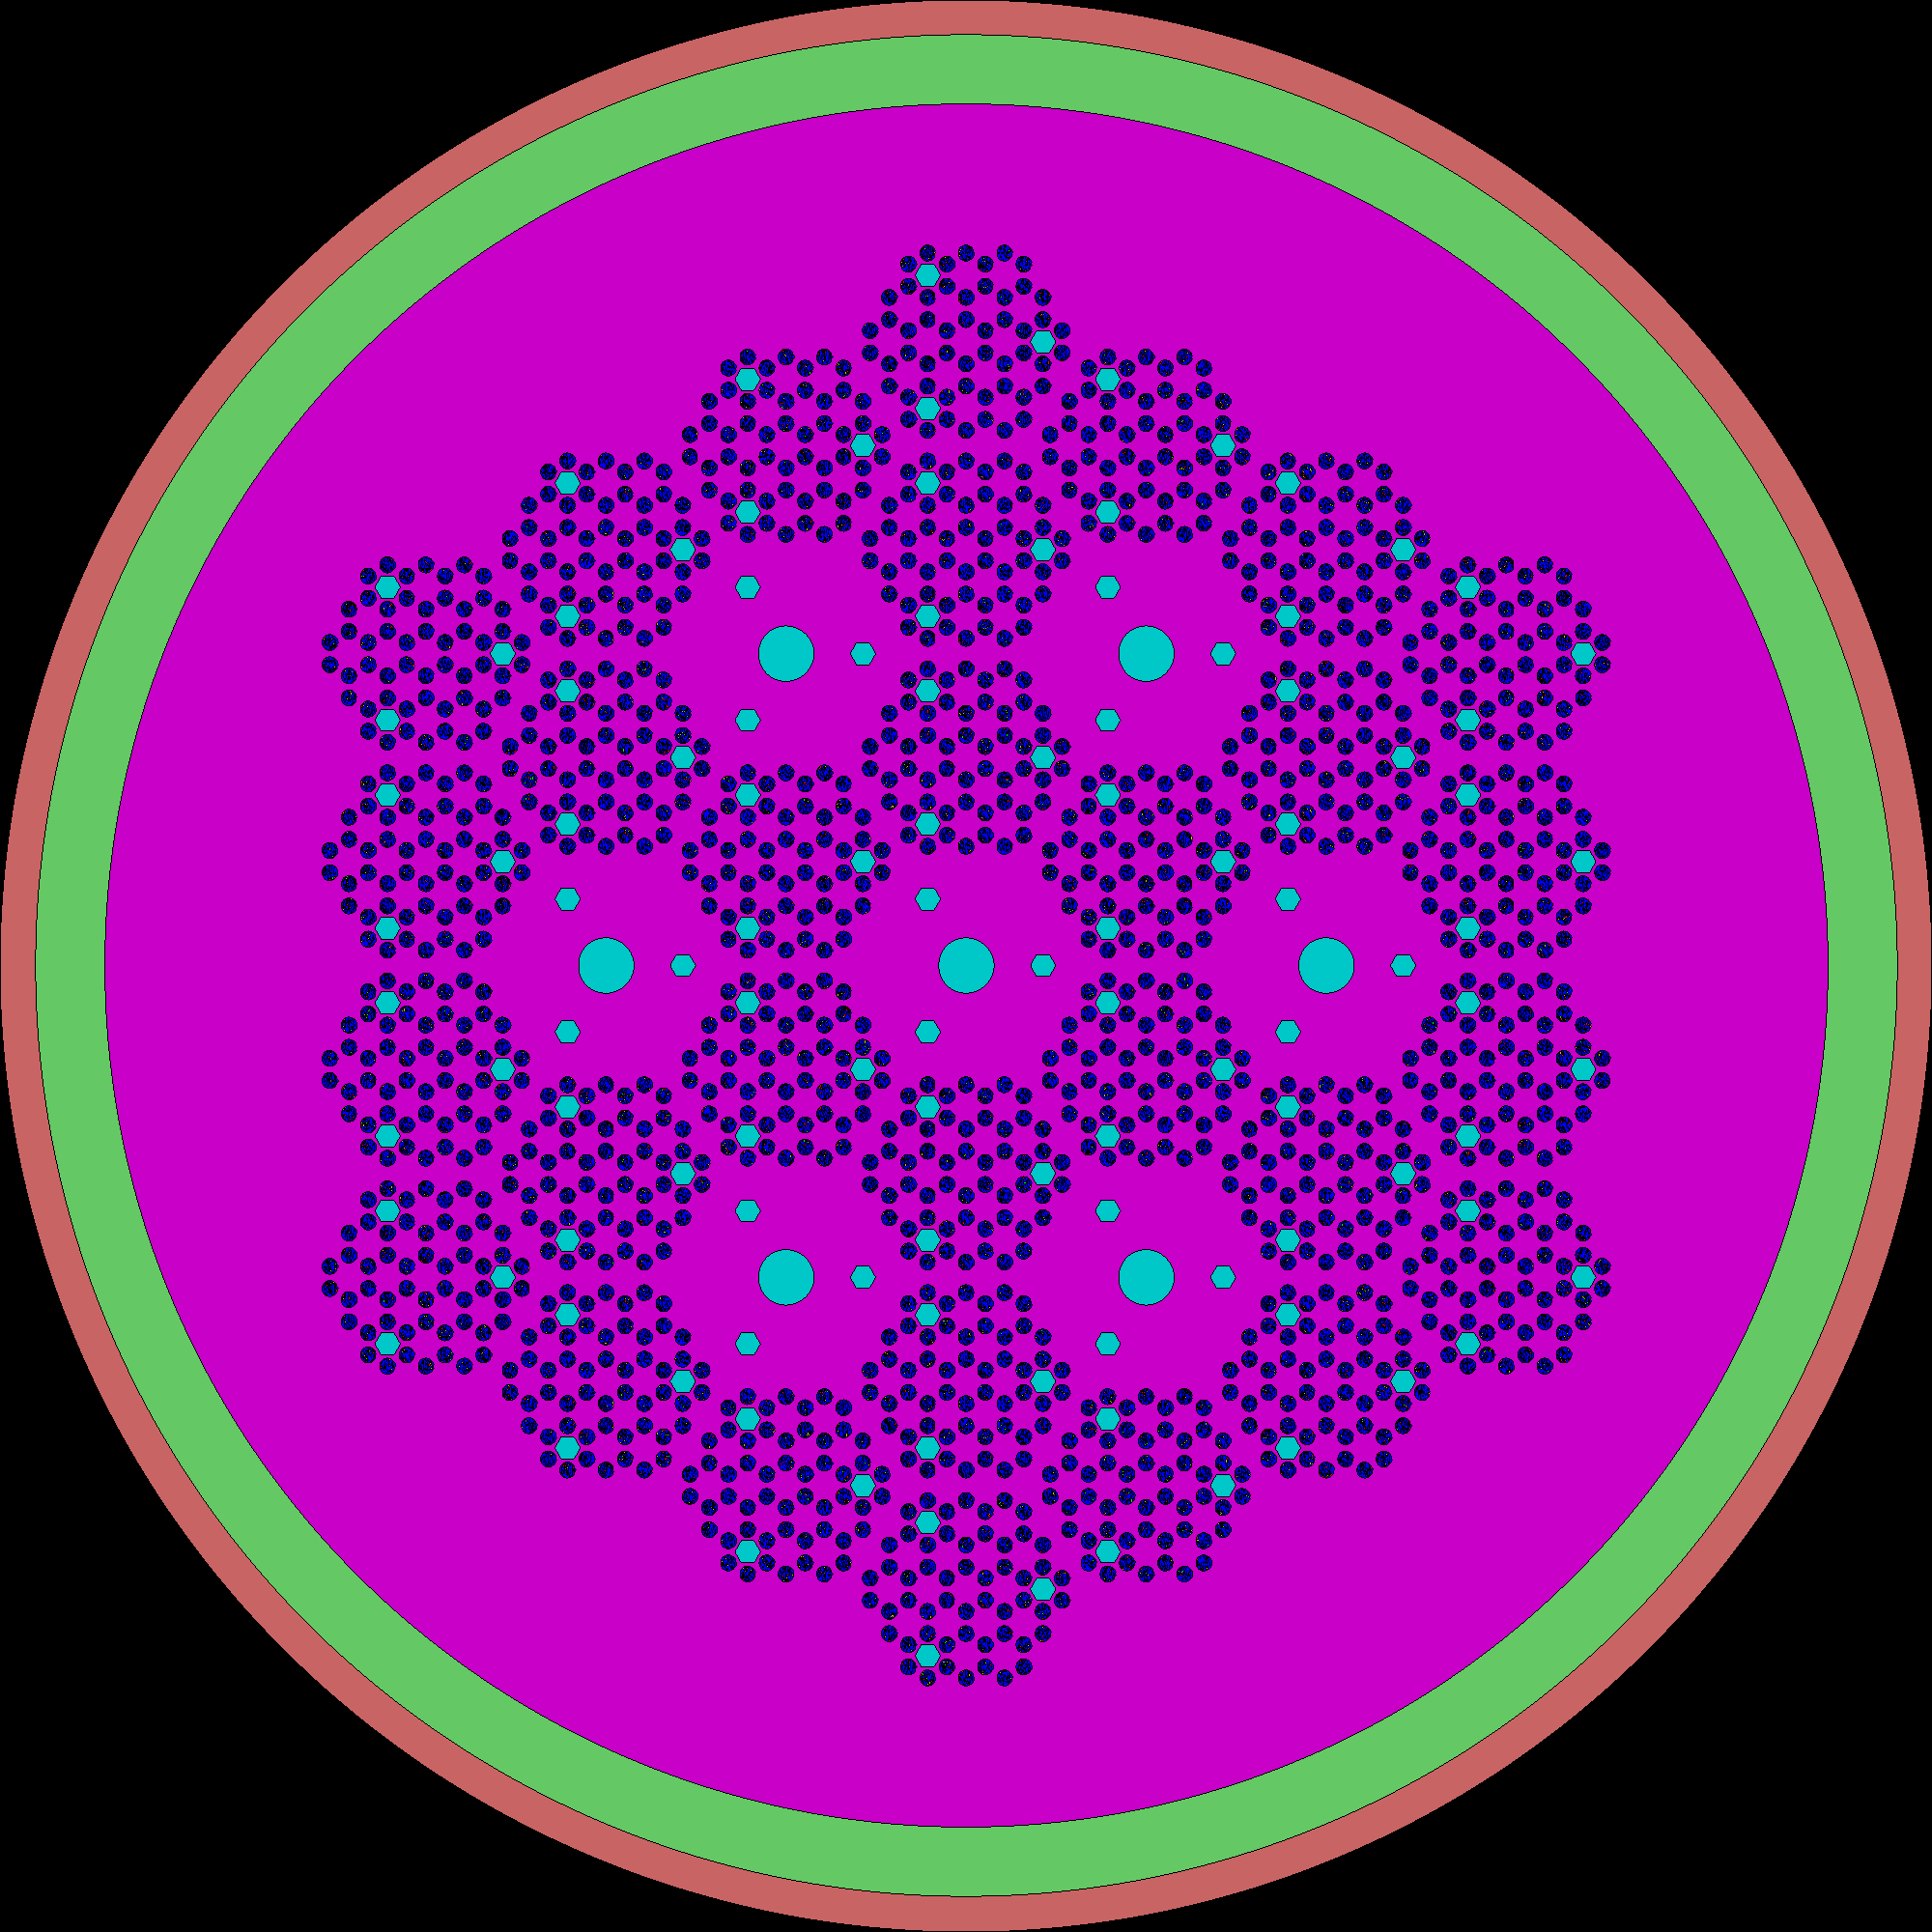
\includegraphics[scale=0.07]{bachmann-mmr_geom1.png}
                \caption{Radial view of the USNC MMR model.}
                \label{fig:mmr_radial}
        \end{subfigure}
        \hfill 
        \begin{subfigure}{0.45\textwidth}
                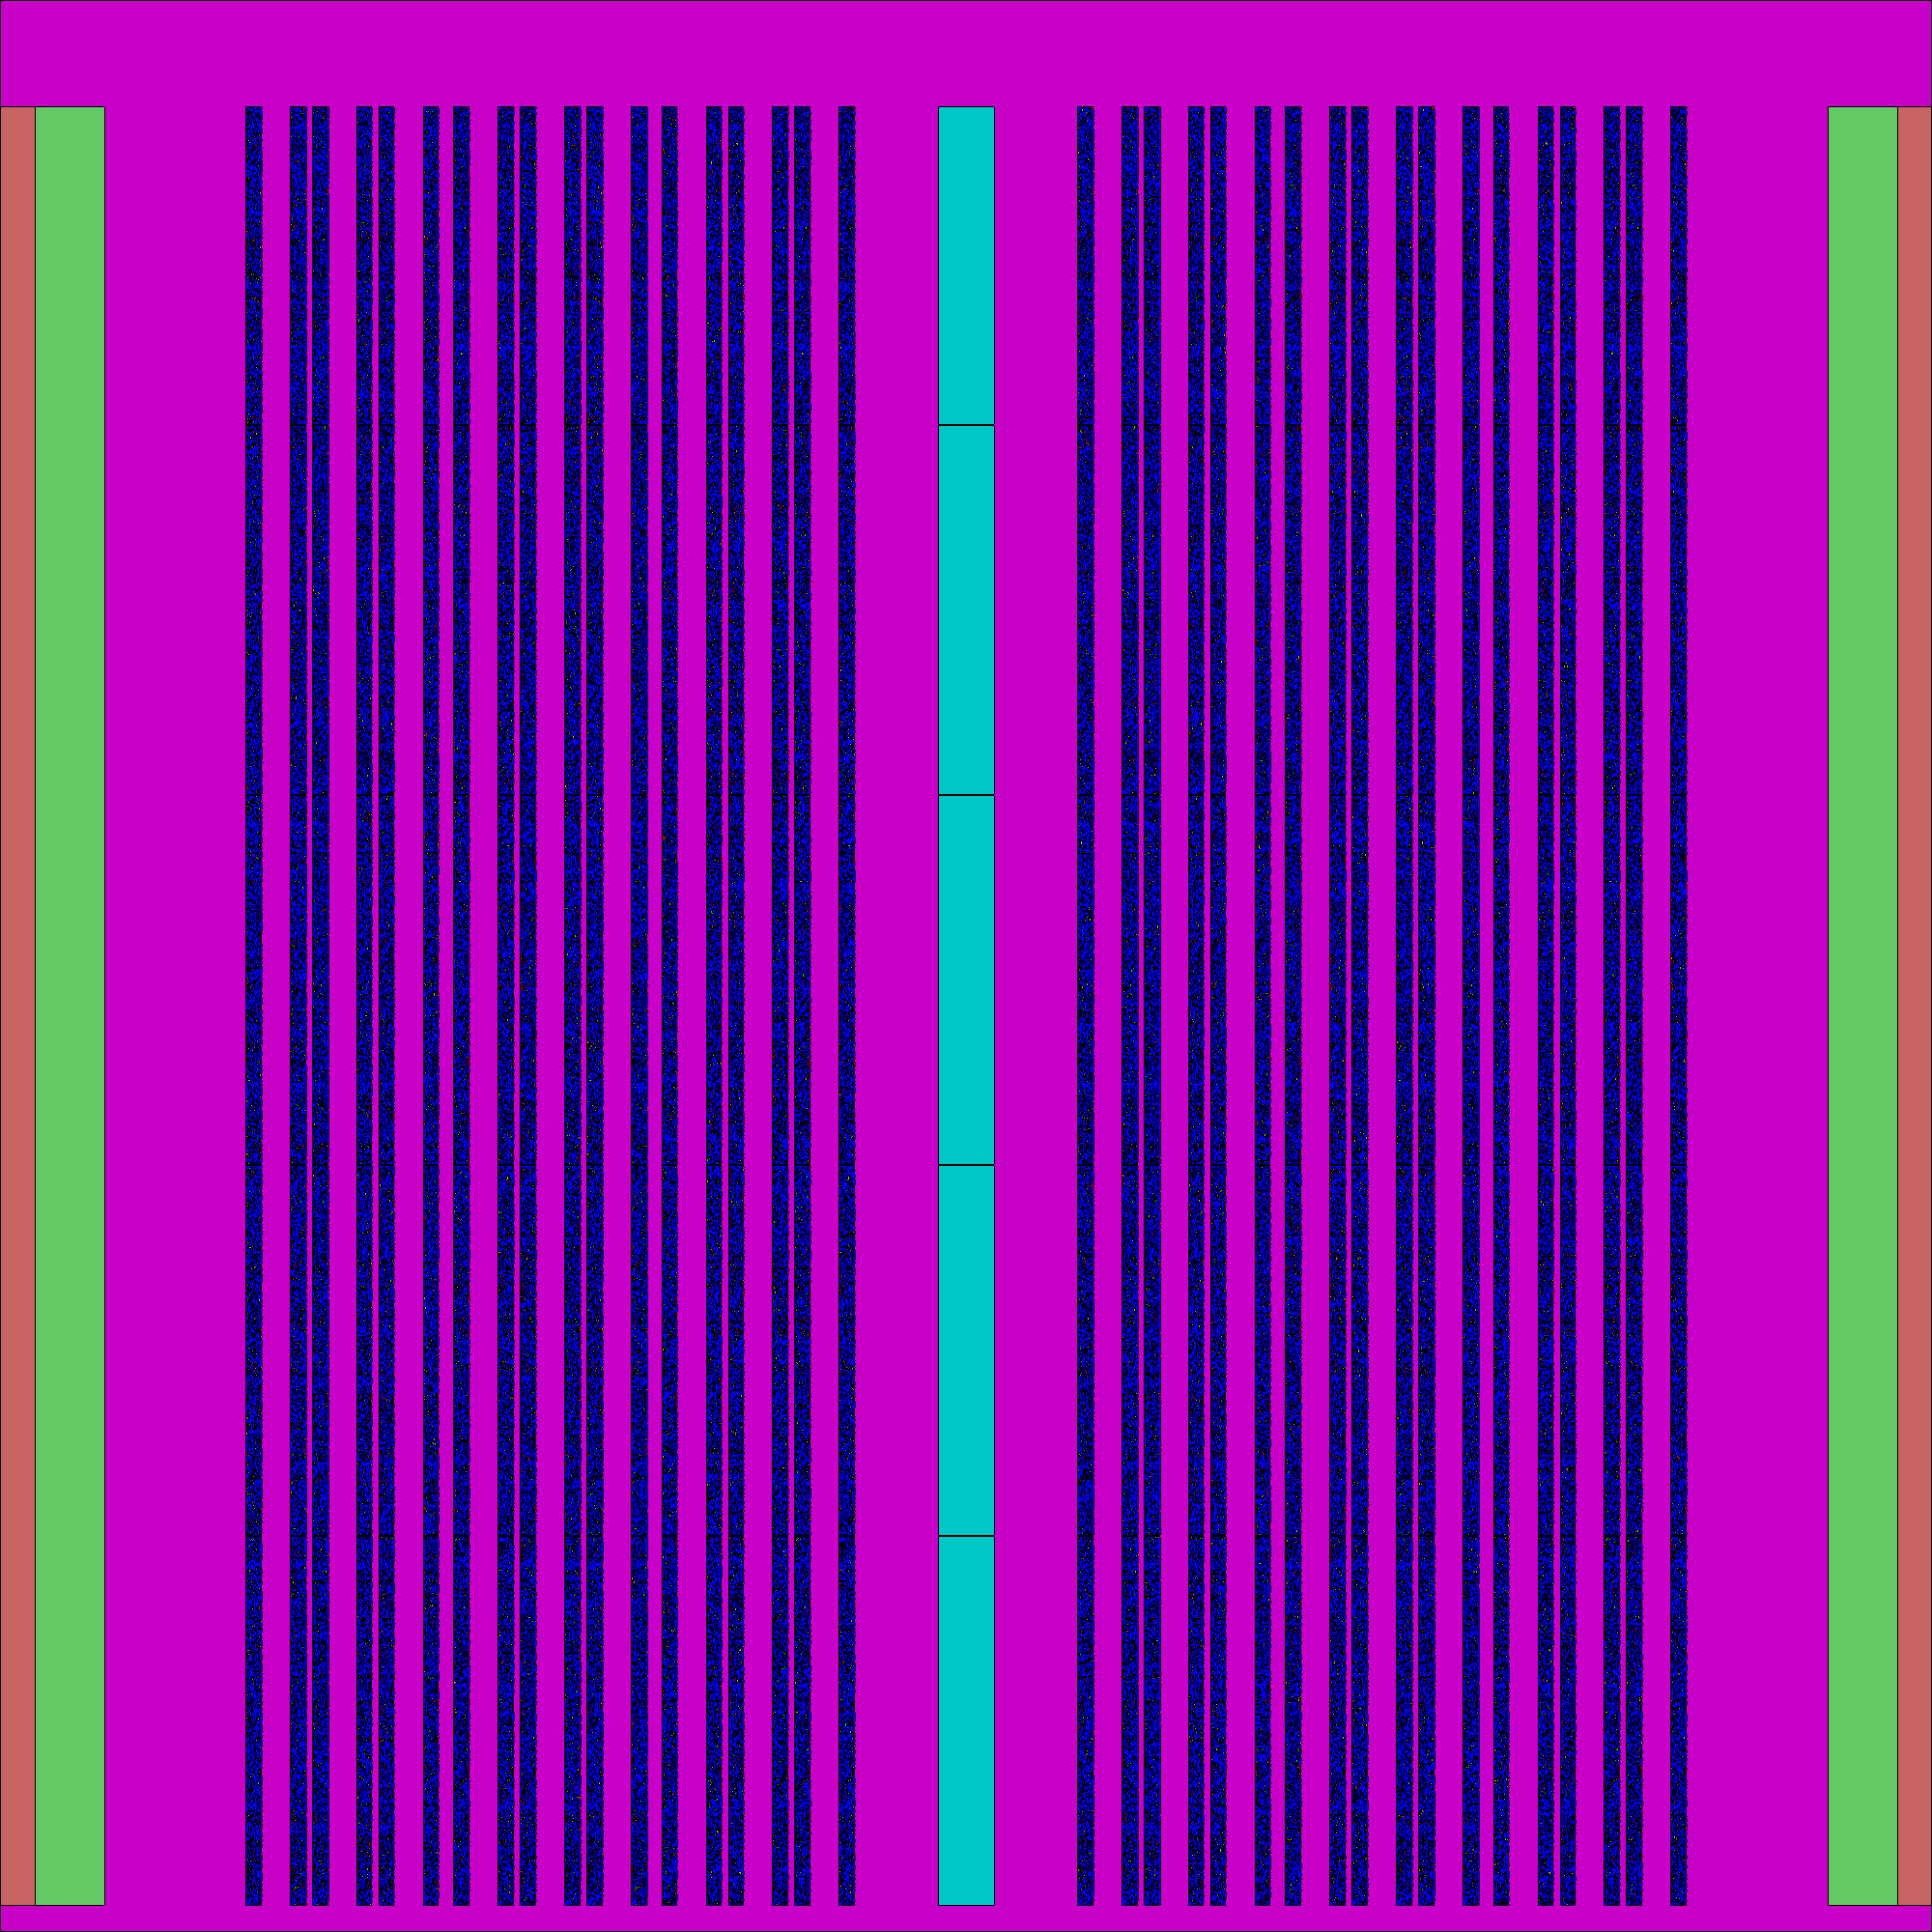
\includegraphics[scale=0.1]{bachmann-mmr_geom3.png}
                \caption{Radial view of the USNC MMR model.}
                \label{fig:mmr_axial}
        \end{subfigure}
        \caption{Geometry of USNC MMR core model in Serpent.}
        \label{fig:mmr_core}
\end{figure}

\section{Results}

The output files from Serpent were parsed and analyzed using the 
``serpentTools'' python package \cite{johnson_serpenttools_2020}. The 
\keff, neutron flux, and \betaEff were output by Serpent. The reactivity 
feedback coefficients were calculated by fitting a linear function to the 
data (material temperature vs reactivity) and propagating error through 
the fit. The neutron flux was divided into two energy groups for 
fast and thermal fluxes. We applied the default two-group structure in Serpent, 
in which the cutoff between the energy groups is 0.625 eV.

\subsection{Xe-100-like reactor}
\subsubsection{k-eff}

\begin{table}
    \centering  
    \caption{\keff value from each fuel composition in the Sangamon200.}
    \label{tab:xe100_keff}
    \begin{tabular}{c c}
        \hline
        Fuel Composition & \keff \\
        \hline
        Pure & \\
        EBR-II & \\
        Y12 & \\
        \hline        
    \end{tabular}
\end{table}

\subsubsection{Neutron flux}

\subsubsection{Beta-eff}
\begin{table}
    \centering  
    \caption{\betaEff value from each fuel composition in the Sangamon200.}
    \label{tab:xe100_betaEff}
    \begin{tabular}{c c}
        \hline
        Fuel Composition & \keff \\
        \hline
        Pure & \\
        EBR-II & \\
        Y12 & \\
        \hline        
    \end{tabular}
\end{table}

\subsubsection{Reactivity coefficients}
\begin{table}
    \centering  
    \caption{Reactivity feedback coefficients from each fuel composition in the Sangamon200.}
    \label{tab:xe100_feedback}
    \begin{tabular}{c c c c c}
        \hline
        & \multicolumn{4}{c}{Feedback Coefficient} \\
        Fuel Composition & Fuel & Moderator & Coolant & Total \\
        \hline
        Pure & \\
        EBR-II & \\
        Y12 & \\
        \hline        
    \end{tabular}
\end{table}

\subsection{MMR-like reactor}
The results of the MMR-like reactor are presented below. The \keff 
values are presented first, followed by the neutron fluxes, the 
\betaEff, and the reactivity coefficients. 

\subsubsection{k-eff}
The fuel composition has a significant effect on the \keff at each 
burnup step, based on the values presented in Table \ref{tab:mmr_keff}.
Using downblended \gls{EBR} or Y12 fuel results in a higher \keff 
at each burnup step, compared with the pure fuel composition.  

\begin{table}
    \centering  
    \caption{\keff value from each fuel composition in the MMR-like model.}
    \label{tab:mmr_keff}
    \begin{tabular}{c c c c}
        \hline
         & \multicolumn{3}{c}{\keff} \\
        Fuel Composition & Beginning of cycle & Mid-cycle & End of cycle \\
        \hline
        Pure & 1.33803 $\pm$ 0.00022 & 1.18042 $\pm$ 0.00024 & 1.05550 $\pm$ 0.00024\\
        EBR-II & 1.49698 $\pm$ 0.00016 & 1.43844 $\pm$ 0.00018 & 1.39386 $\pm$ 0.00016\\
        Y12 & 1.49666 $\pm$ 0.00017 & 1.43894 $\pm$ 0.00016 & 1.39392 $\pm$ 0.00015\\
        \hline        
    \end{tabular}
\end{table}



\subsubsection{Neutron flux}

Using the downblended fuel compositions results in depressions in the 
thermal (Figure \ref{fig:mmr_thermal_axial}) and fast (Figure 
\ref{fig:mmr_fast_axial}) neutron fluxes through the center of the core. 
We observed a similar depression in the axial flux at the other 
burnup steps. 


\begin{figure}
    \centering 
    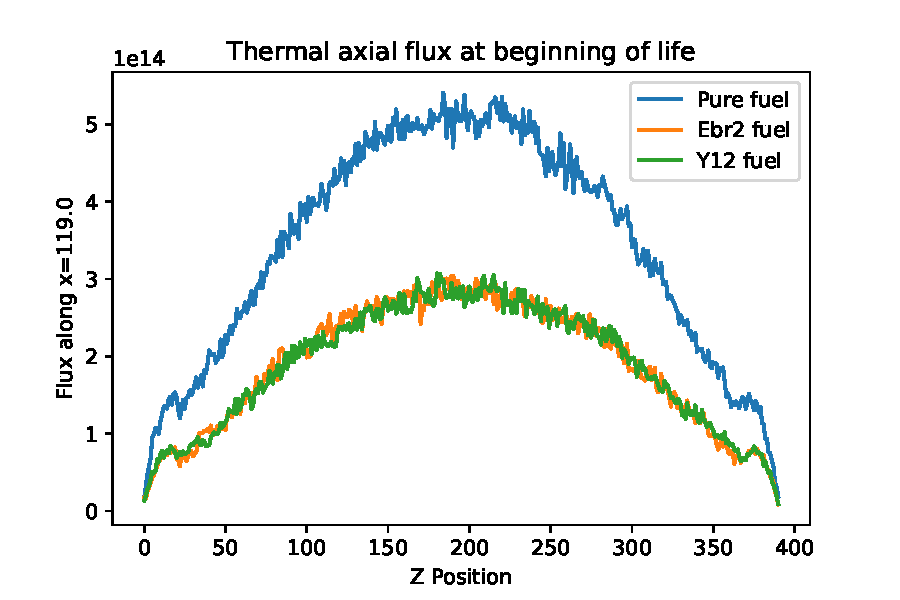
\includegraphics[trim = 20 0 0 0,clip,scale=0.8]{thermal_axial_flux_0.pdf}
    \caption{Thermal, axial neutron flux through the MMR-like reactor using 
    each fuel composition at the beginning of life (0 MWd/kgU burnup).}
    \label{fig:mmr_thermal_axial}
\end{figure}

\begin{figure}
    \centering 
    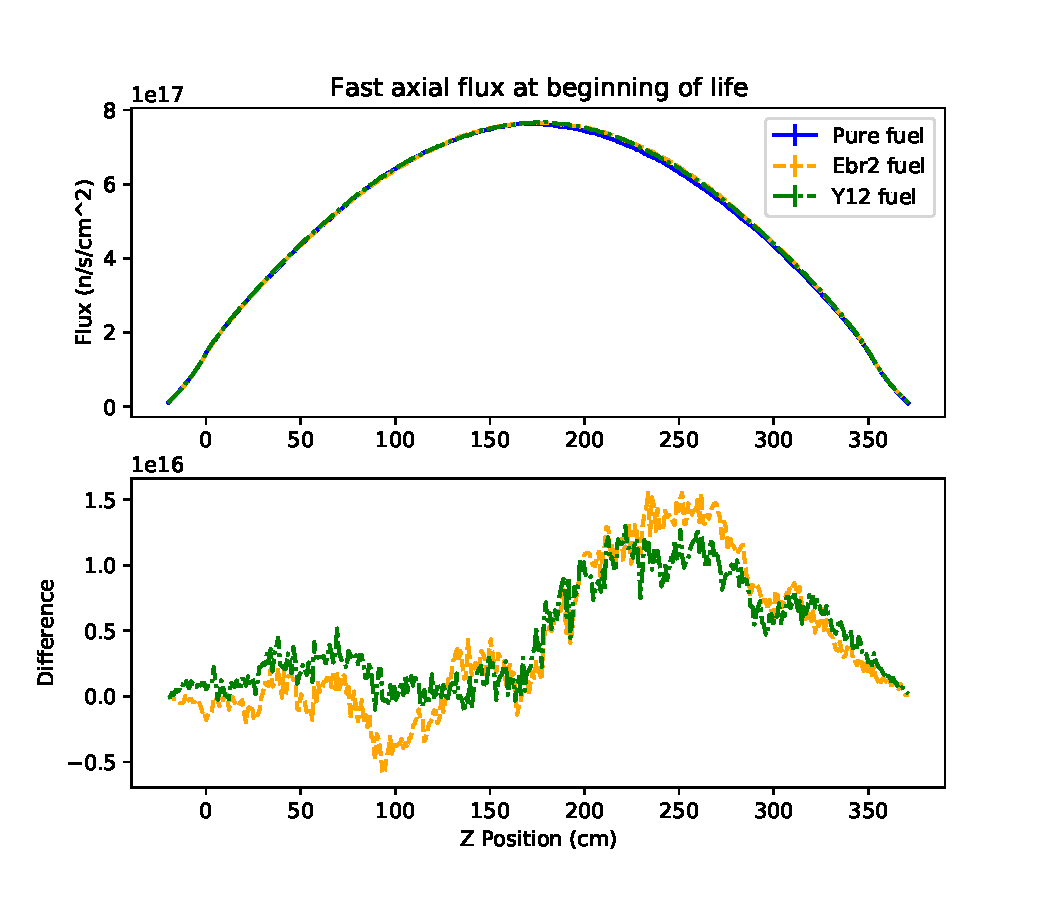
\includegraphics[trim = 20 0 0 0,clip,scale=0.8]{fast_axial_flux_0.pdf}
    \caption{Fast, axial neutron flux through the MMR-like reactor using 
    each fuel composition at the beginning of life (0 MWd/kgU burnup).}
    \label{fig:mmr_fast_axial}
\end{figure}

Additionally, using the downblended fuel compositions resulted in a 
depressed neutron flux (Figures \ref{fig:mmr_thermal_radial} and 
\ref{fig:mmr_fast_radial}) in the radial direction. However, the 
depression in the radial flux is a smaller magnitude than the depression 
in the axial flux. 

\begin{figure}
    \centering 
    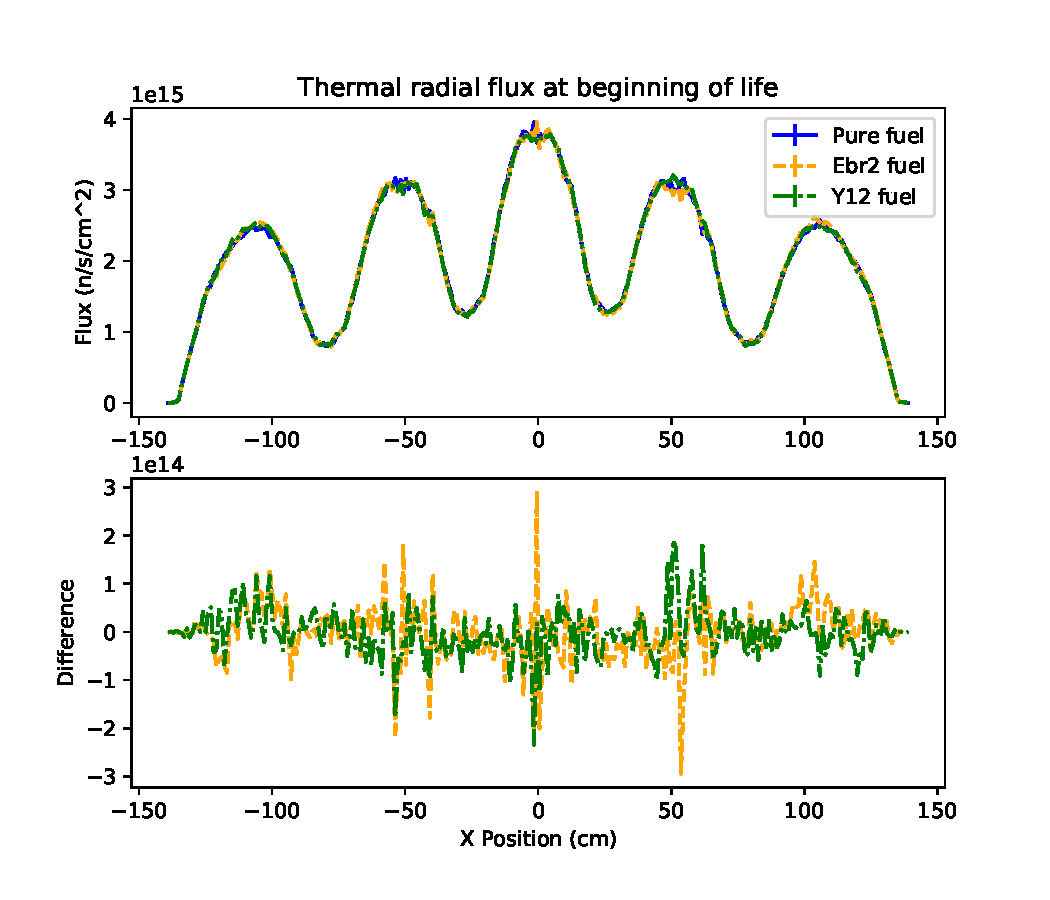
\includegraphics[trim = 20 0 0 0,clip,scale=0.8]{thermal_radial_flux_0.pdf}
    \caption{Thermal, radial neutron flux through the MMR-like reactor using 
    each fuel composition at the beginning of life (0 MWd/kgU burnup).}
    \label{fig:mmr_thermal_radial}
\end{figure}

\begin{figure}
    \centering 
    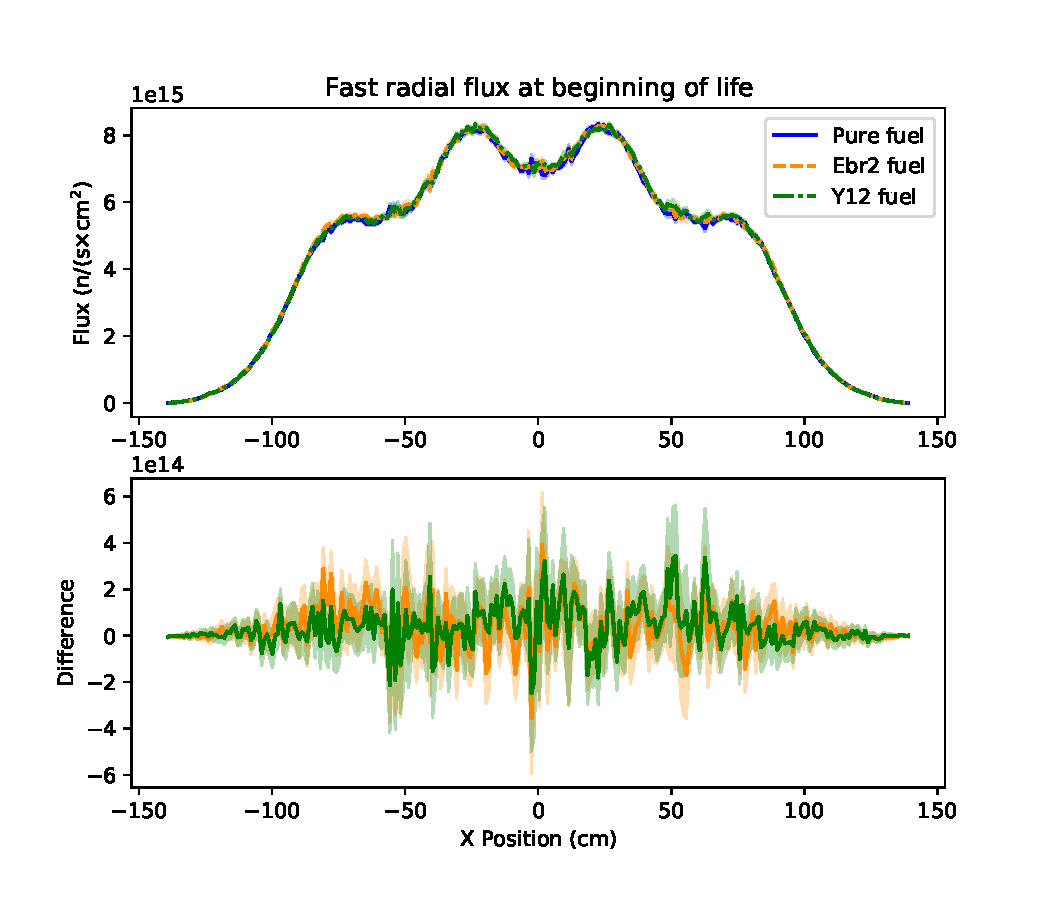
\includegraphics[trim = 20 0 0 0,clip,scale=0.8]{fast_radial_flux_0.pdf}
    \caption{Fast, radial neutron flux through the MMR-like reactor using 
    each fuel composition at the beginning of life (0 MWd/kgU burnup).}
    \label{fig:mmr_fast_radial}
\end{figure}


\subsubsection{Beta-eff}
\begin{table}
    \centering  
    \caption{\betaEff value from each fuel composition in the MMR-like model.}
    \label{tab:mmr_betaEff}
    \begin{tabular}{c c c c}
        \hline
         & \multicolumn{3}{c}{\betaEff} \\
        Fuel Composition & Beginning of cycle & Mid-cycle & End of cycle \\
        \hline
        Pure & 0.00549 $\pm$ 0.00610\\
        EBR-II & 0.00649 $\pm$ 0.00533\\
        Y12 & 0.00644 $\pm$ 0.00475\\
        \hline        
    \end{tabular}
\end{table}


\subsubsection{Reactivity coefficients}

\begin{table}
    \centering  
    \caption{Fuel temperature reactivity feedback coefficients (pcm/K) from 
    each fuel composition in the MMR.}
    \label{tab:mmr_fuel_feedback}
    \begin{tabular}{c c c c}
        \hline
        & \multicolumn{3}{c}{Burnup step} \\
        \hline
        Fuel composition & Beginning of cycle & Mid-cycle & End of cycle \\\hline
        Pure & -2.968 $\pm$ 0.053 & -3.955 $\pm$ 0.144 & -4.613 $\pm$ 0.285\\
        EBR-II & -1.183 $\pm$ 0.041 & -1.191 $\pm$ 0.164 & -1.327 $\pm$ 0.071\\
        Y12 & -1.266 $\pm$ 0.034 & -1.334 $\pm$ 0.026 & -0.989 $\pm$ 0.075\\
        \hline        
    \end{tabular}
\end{table}

\begin{table}
    \centering  
    \caption{Moderator temperature reactivity feedback coefficients from each 
    fuel composition in the MMR.}
    \label{tab:mmr_moderator_feedback}
    \begin{tabular}{c c c c}
        \hline
        & \multicolumn{3}{c}{Burnup step} \\
        \hline
        Fuel composition & Beginning of cycle & Mid-cycle & End of cycle \\\hline
        Pure & -0.871 $\pm$ 0.062 & -1.426 $\pm$ 0.227 & -2.215 $\pm$ 0.258\\
        EBR-II & -0.426 $\pm$ 0.035 & -0.376 $\pm$ 0.173 & -0.336 $\pm$ 0.063\\
        Y12 & -0.354 $\pm$ 0.063 & -0.139 $\pm$ 0.069 & -0.155 $\pm$ 0.100\\
        \hline        
    \end{tabular}
\end{table}

\begin{table}
    \centering  
    \caption{Coolant temperature reactivity feedback coefficients from each fuel composition in the MMR.}
    \label{tab:mmr_coolant_feedback}
    \begin{tabular}{c c c c}
        \hline
        & \multicolumn{3}{c}{Burnup step} \\
        \hline
        Fuel composition & Beginning of cycle & Mid-cycle & End of cycle \\\hline
        Pure & 0.001 $\pm$ 0.067 & -0.085 $\pm$ 0.086 & 0.280 $\pm$ 0.152\\
        EBR-II & 0.083 $\pm$ 0.089 & -0.139 $\pm$ 0.149 & 0.046 $\pm$ 0.076\\
        Y12 & 0.000 $\pm$ 0.048 & 0.001 $\pm$ 0.077 & -0.029 $\pm$ 0.067\\
        \hline        
    \end{tabular}
\end{table}

\begin{table}
    \centering  
    \caption{Total temperature reactivity feedback coefficients from each fuel composition in the MMR.}
    \label{tab:mmr_total_feedback}
    \begin{tabular}{c c c c}
        \hline
        & \multicolumn{3}{c}{Burnup step} \\
        \hline
        Fuel composition & Beginning of cycle & Mid-cycle & End of cycle \\\hline
        Pure & -3.956 $\pm$ 0.106 & -5.473 $\pm$ 0.272 & -6.687 $\pm$ 0.337\\
        EBR-II & -1.554 $\pm$ 0.051 & -1.321 $\pm$ 0.1887 & -1.446 $\pm$ 0.159\\
        Y12 & -1.436 $\pm$ 0.116 & -1.450 $\pm$ 0.204 & -1.521 $\pm$ 0.074\\
        \hline        
    \end{tabular}
\end{table}
\section{Conclusions}
To adapt to the sudden need for \gls{HALEU}, the \gls{DOE} is 
considering downblending some stockpiles of \gls{HEU} to produce 
fuel for reactors. However, the presence of other uranium isotopes 
in the fuel can introduce affects on the reactor performance that are 
not typically seen in fuel produced from enriching natural 
uranium. To investigate if these effects can significantly impact 
reactor performance, we simulated the reactor physics of 
an Xe-100-like reactor and an \gls{MMR}-like reactor using 
three different \gls{HALEU} compositions. The \gls{HALEU} 
compositions were based on pure \gls{HALEU} (only $^{235}$U and 
$^{238}$U), downblended \gls{HEU} from \gls{EBR} stockpiles, 
and downblended \gls{HEU} from the Y-12 National Security Complex. 
We compared the performance of the different fuel compositions
based on the \keff, \betaEff, energy- and spatially-dependent 
neutron flux, and the fuel, moderator, coolant, and total reactivity 
temperature feedback coefficients. 

In the Xe-100-like model, the impure fuel compositions resulted 
in higher \keff values, which suggests that additional neutron 
poisons may be needed during operation to control the reactivity 
in the core. The \betaEff values when using the impure fuel are 
lower than the \betaEff from the pure fuel, which suggests that 
reactivity control mechanisms may not be as effective when using 
the impure fuels. The impure fuels resulted in a depression in the 
thermal neutron flux across the active region of the core. There is 
is also an asymmetry in the axial fluxes that is partially because 
of the different fuel compositions and partially because of 
pebble placement in the core. Finally, the impure fuels 
lead to reactivity feedback coefficients that are more negative 
or within error of the values from the pure fuel. This result 
suggests that these fuel compositions does not significanty effect 
these metrics or would place the reactor in a safer operating state. 

In the \gls{MMR}-like model, the impure fuels result in smaller 
\keff values at each burnup step, but do not prevent the reactor 
from still being critical at \gls{EOL}. While this result may effect 
how neutron poisons are used during operation, it shows that 
the 20 year cycle time of the reactor is still possible with 
any of these \gls{HALEU} compositions. The \betaEff values from 
the different \gls{HALEU} compositions are all within error 
of each other at each burnup step, suggesting that the fuel 
composition does not significantly impact this metric for this 
reactor design. The impure fuels lead to larger fluxes in the 
fast energy range,, compared with the pure fuel, and the 
radially-dependent flux is dependent on proximity to fuel pin 
and coolant channels in the core. Most of the reactivity feedback 
coefficients from the different fuel compositions are within 
error of each other. The one exception is the coolant feedback 
coefficient, but the smaller absolute value of this coefficient 
compared with the others means that it has a smaller effect on 
the temperature-dependent reactivity changes in the core. These
results suggest that these different \gls{HALEU} compositions 
do not have a significant effect on the performance of this 
reactor design, and would not prevent it from operating in 
a safe state. 



\subsection{Future Work}
The work presented here is an initial start to understanding the impacts 
of using downblended \gls{HEU} in reactors. To more completely understand 
the effects of using these fuel compositions, one would need to 
update the models to more accurately capture each reactor design. This 
includes the reactor geometries, using non-homogeneous fuel materials, 
and nonhomogeneous material temperatures. Each of these model components 
limit the accuracy of the work completed here, and accurate depictions 
of them will provide more detail on the effects of using each fuel composition. 

Additionally, the Xe-100-like model assumes an equilibrium state. 
However, downblended \gls{HEU} may be used to create fuel for start up 
cores. Therefore, analysis of these compositions in the the Xe-100 
design in a start up core configuration would be more beneficial to 
understanding potential limitations of these fuel composisions 
to initially fuel reactors while developing infrastructure to 
enrich natural uranium to produce \gls{HALEU}.

Finally, neither of the companies designing these reactors have 
announced intentions to use downblended \gls{HEU}, but Oklo has announced 
intentions of using the downblended \gls{EBR} fuel for their Aurora reactor 
design \textbf{Find citation}. Therefore, a more practical investigation 
would 
be to apply this methodology to that reactor design, especially 
since it has some notable design differences to the reactors considered 
here, namely that it is a fast spectrum reactor. 

\section{Acknowledgments}
This material is based upon work supported under a University Nuclear 
Leadership Program Graduate
Fellowship. 

Argonne's efforts were sponsored by the U.S. Department of 
Energy under Contract DE-AC02-06CH11357.

The authors thank Nathan Glaser of the Advanced Reactors and 
Fuel Cycles Group for his review of this publication. 

\bibliography{bibliography}

% Prof. Huff discourages appendices in journal articles.
% But, if you must, include one like so:
%\pagebreak
%
\appendix
\section{}


\end{document}
